\chapter{Implementation}
As par the implementation part is concern we required certain modules to be integrate to form the whole system or tool. Form the implementation point of view this tool is divided into following modules .
\begin{itemize}
\item Input Source File
\item Tokenization and Parsing
\item Generating Tables
\item Analysis
\item Output
\end{itemize}

\section{Input Source File}

A normal multithreaded program is given as input with critical sections. This file is first compiled to check for errors and only when it is compiled error free; it heads to the next stage.
\begin{figure}[H]
\centering
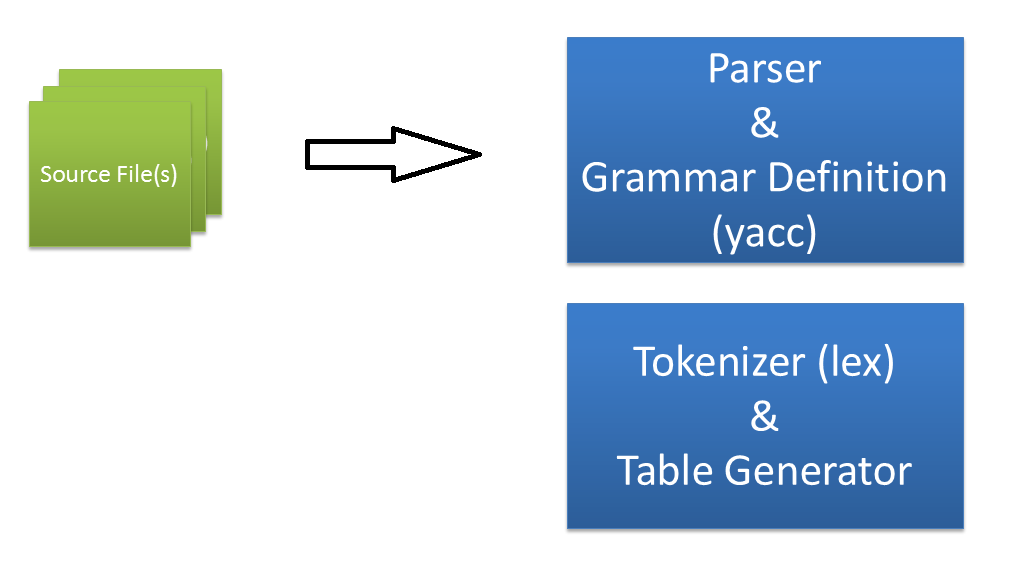
\includegraphics[scale=0.4]{input.png}
\caption{Input}
\label{<<Label>>}
\end{figure}

\section{Tokenization and Parsing}

%Add Description here.. 
Module of the Tokenization and Parsing is i

\begin{figure}[H]
\centering
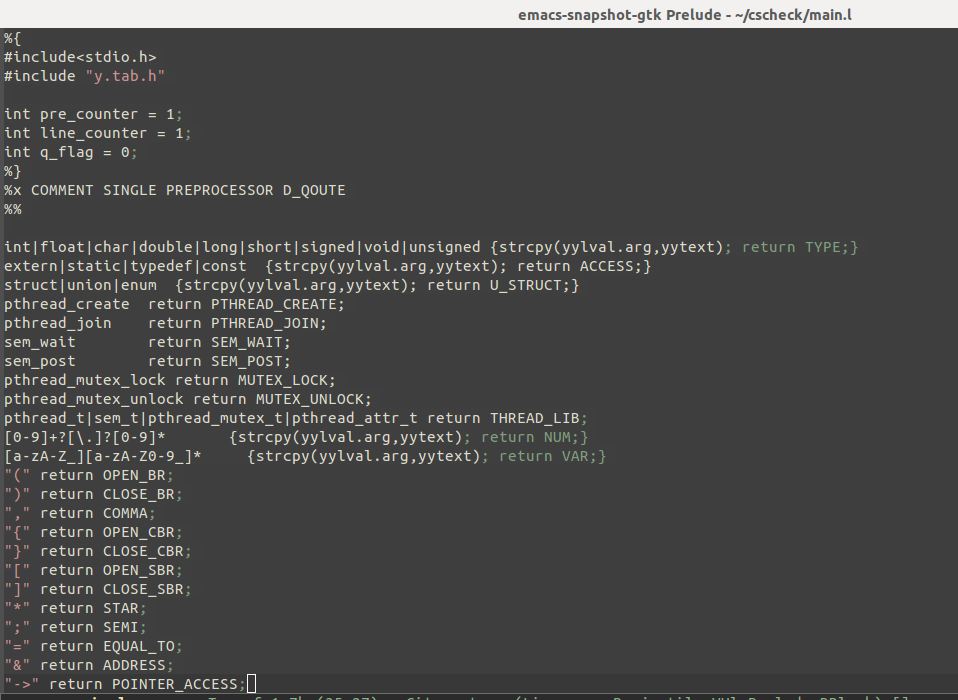
\includegraphics[scale=0.4]{Snaps/main_l_1.png}
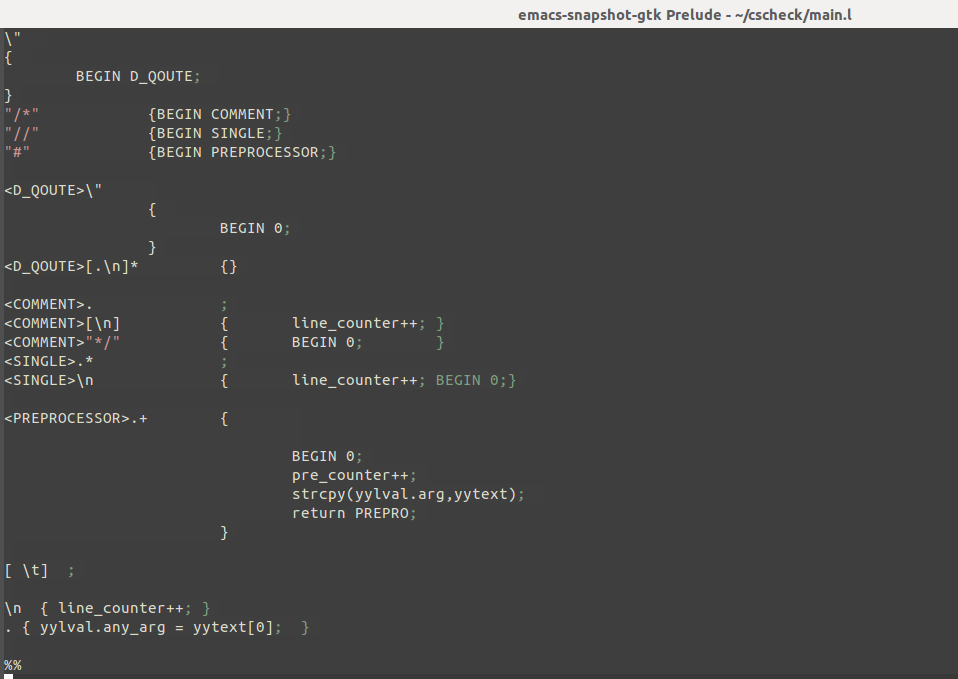
\includegraphics[scale=0.4]{Snaps/main_l_2.png}
\caption{Tokens}
\label{<<Label>>}
\end{figure}
\newpage
\section{Generating Tables}
%Add Description here..
Header contains structures for handling critical section and declarations	
for genrating tables.								
											
Structures defined contains the information extracted by the parser.		
It contains the important parameters of C program which are helpful		
in finding critical section. Tables generated from structures will		
contain the information extracted from parser.	
\begin{figure}[H]
\centering
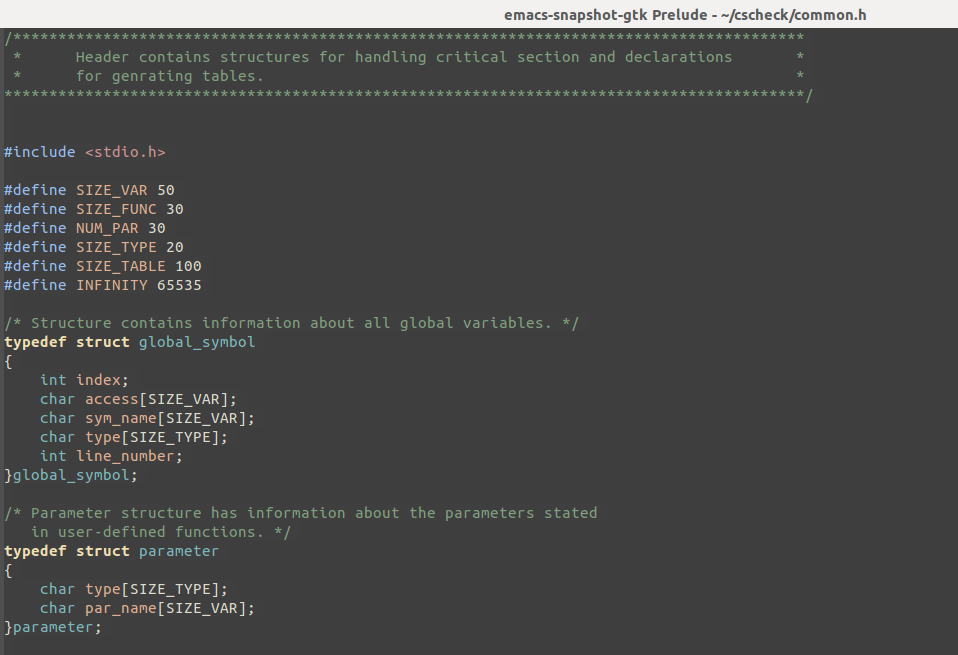
\includegraphics[scale=0.4]{Snaps/common_1.png}
\label{<<Label>>}
\end{figure}

\begin{figure}[H]
\centering
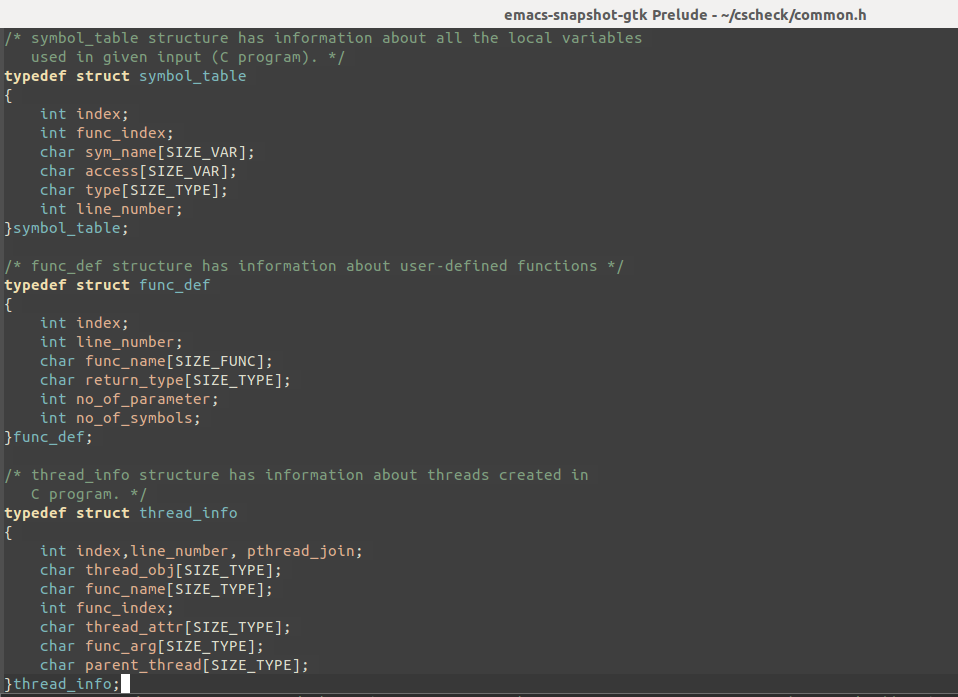
\includegraphics[scale=0.4]{Snaps/common_2.png}
\label{<<Label>>}
\end{figure}

\begin{figure}[H]
\centering
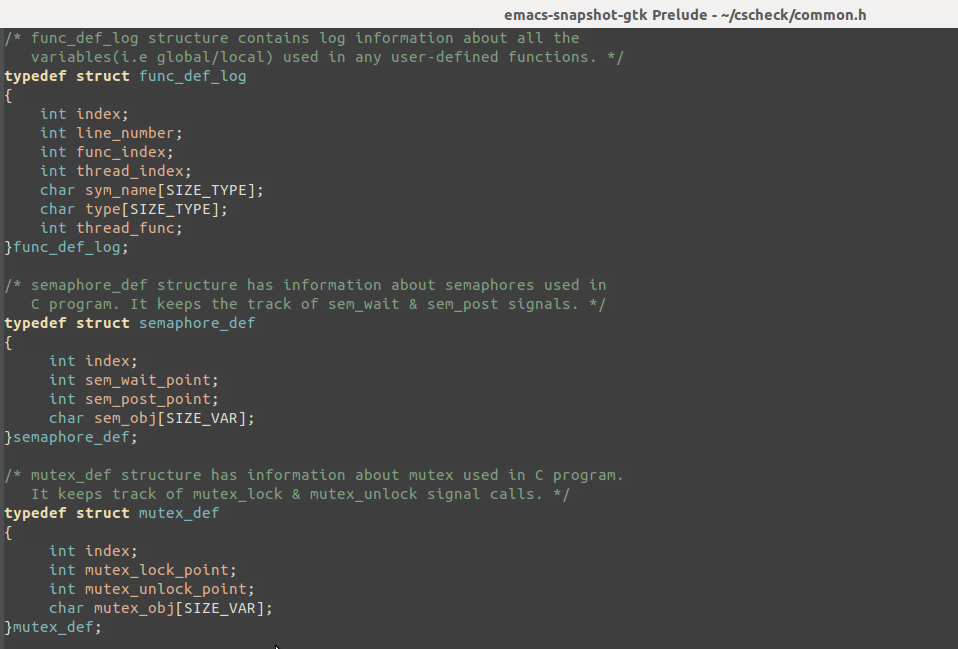
\includegraphics[scale=0.4]{Snaps/common_3.png}
\label{<<Label>>}
\end{figure}

\begin{figure}[H]
\centering
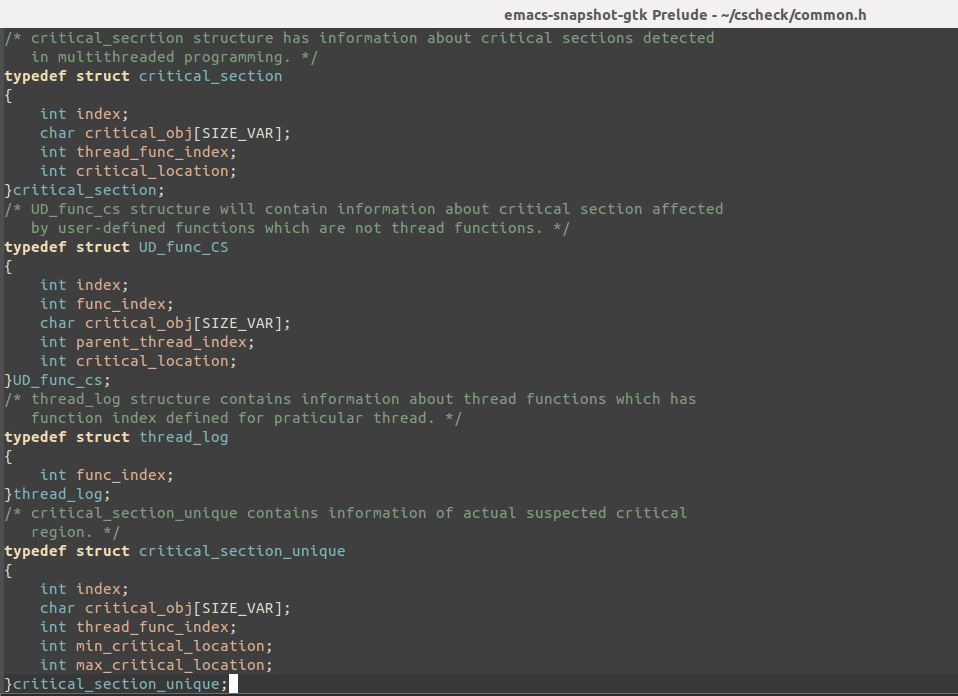
\includegraphics[scale=0.4]{Snaps/common_4.png}
\label{<<Label>>}
\end{figure}

\begin{figure}[H]
\centering
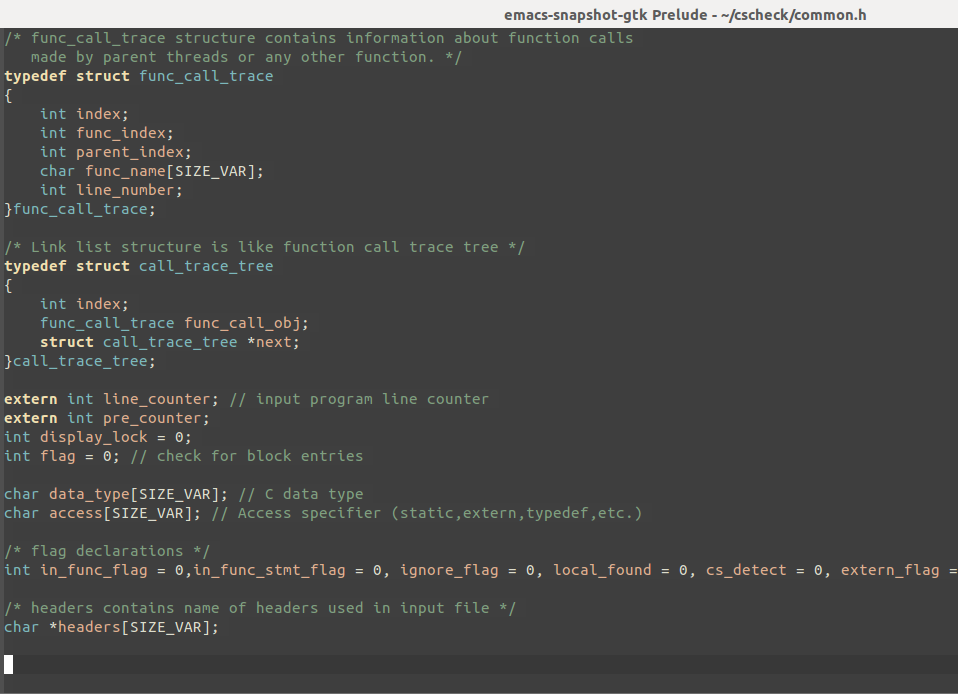
\includegraphics[scale=0.4]{Snaps/common_5.png}
\label{<<Label>>}
\end{figure}

\begin{figure}[H]
\centering
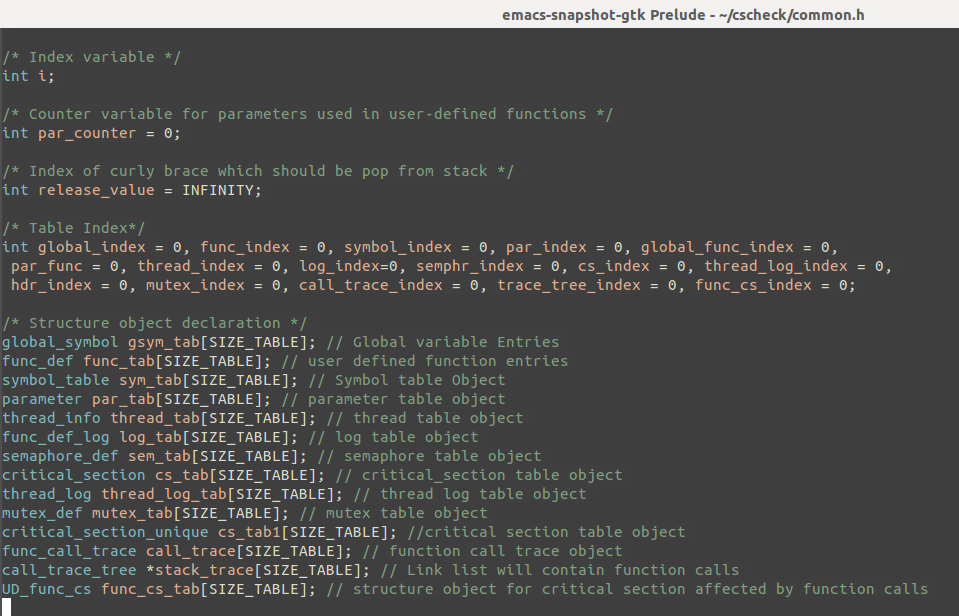
\includegraphics[scale=0.4]{Snaps/common_6.png}
\caption{Structures of all the tables}
\label{<<Label>>}
\end{figure}





\section{Analysis}
%Add Description here..
Program contains stack opration which is used for handling curly brace.

Main purpose of handling curly brace is to identify equal occurence of
opening and closing curly brace. This would help to identify inner functions
and can be helpful to identify the enttries of shadowing global variables.
\begin{figure}[H]
\centering
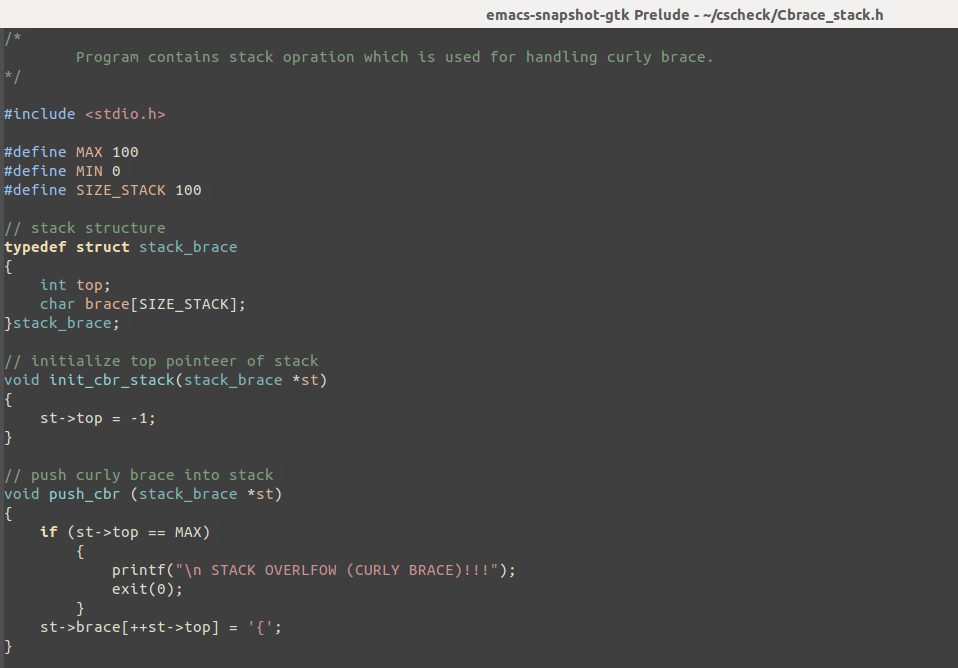
\includegraphics[scale=0.4]{Snaps/stacktrace_1.png}
\caption{Cbrace\_stack.h}
\label{<<Label>>}
\end{figure}

Program contains generation of tables, processing of tables and displaying	
output.										
 											
Tables are generated using the information generated by grammar written in	
yacc file. Functions are written to analyze those tables and generate		
required output. The information generated by these functions are stored in     
proper data structures and display functions are written to view the required   
information stored in those structures. 

\begin{figure}[H]
\centering
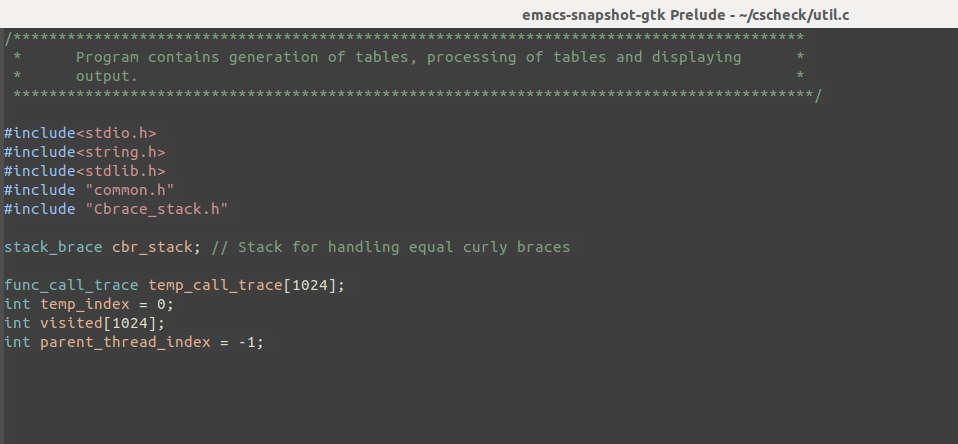
\includegraphics[scale=0.4]{Snaps/util_1.png}
\label{<<Label>>}
\end{figure}

\begin{figure}[H]
\centering
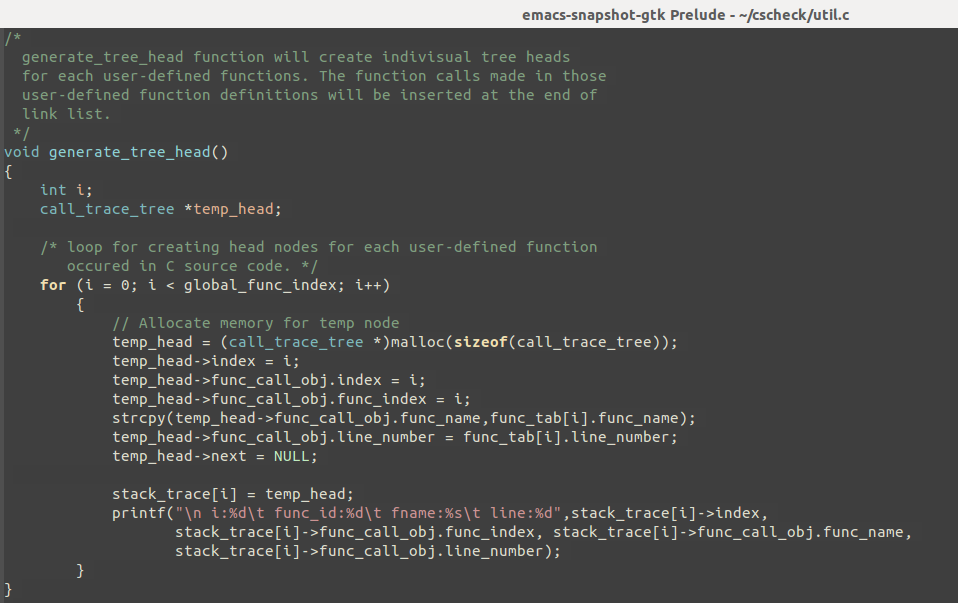
\includegraphics[scale=0.4]{Snaps/util_5.png}
\label{<<Label>>}
\end{figure}

\begin{figure}[H]
\centering
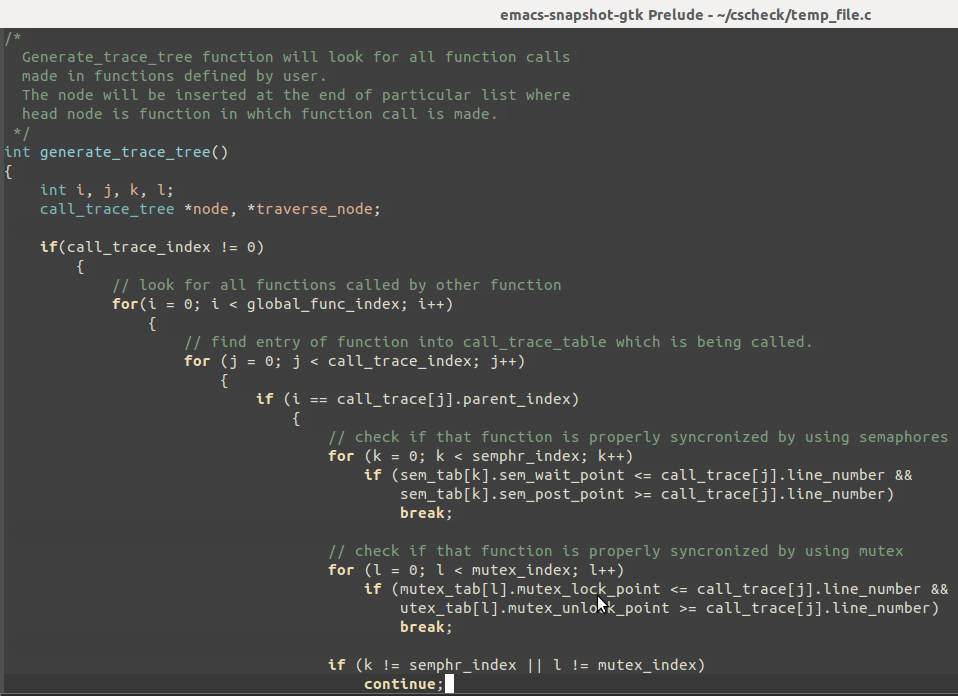
\includegraphics[scale=0.4]{Snaps/util_6.png}
\label{<<Label>>}
\end{figure}

\begin{figure}[H]
\centering
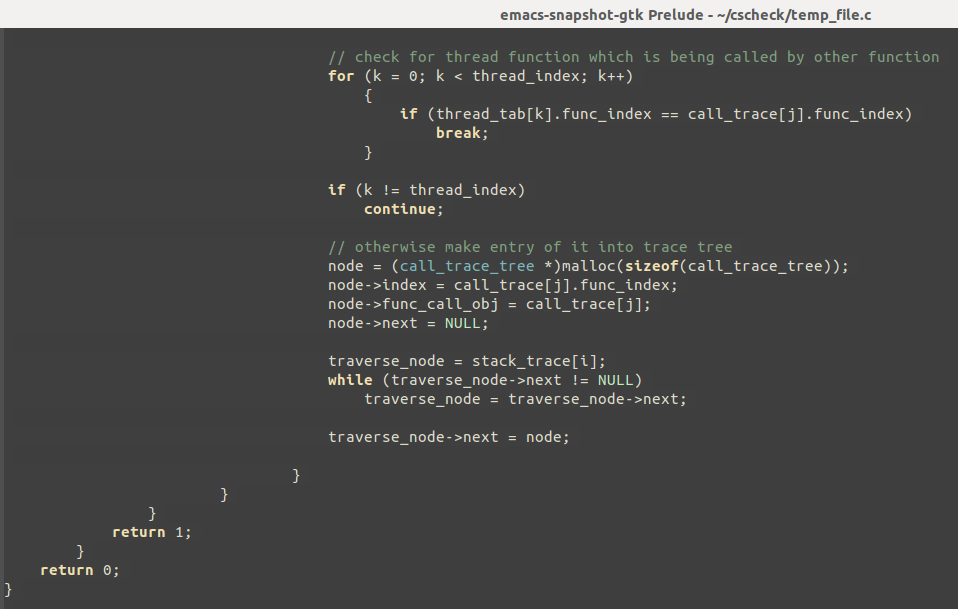
\includegraphics[scale=0.4]{Snaps/util_7.png}
\label{<<Label>>}
\end{figure}

\begin{figure}[H]
\centering
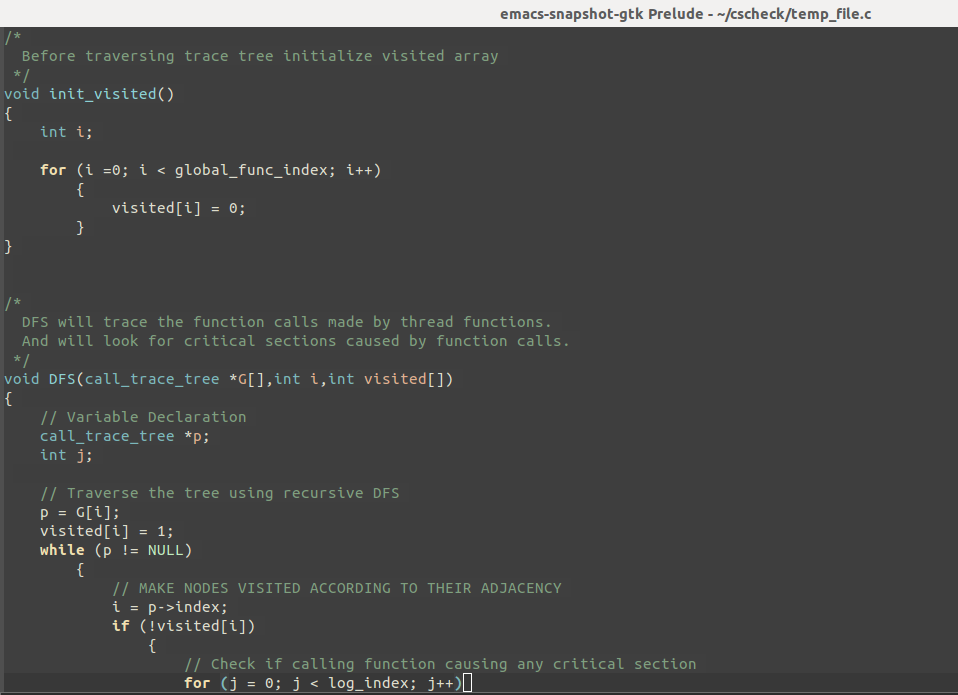
\includegraphics[scale=0.4]{Snaps/util_8.png}
\label{<<Label>>}
\end{figure}

\begin{figure}[H]
\centering
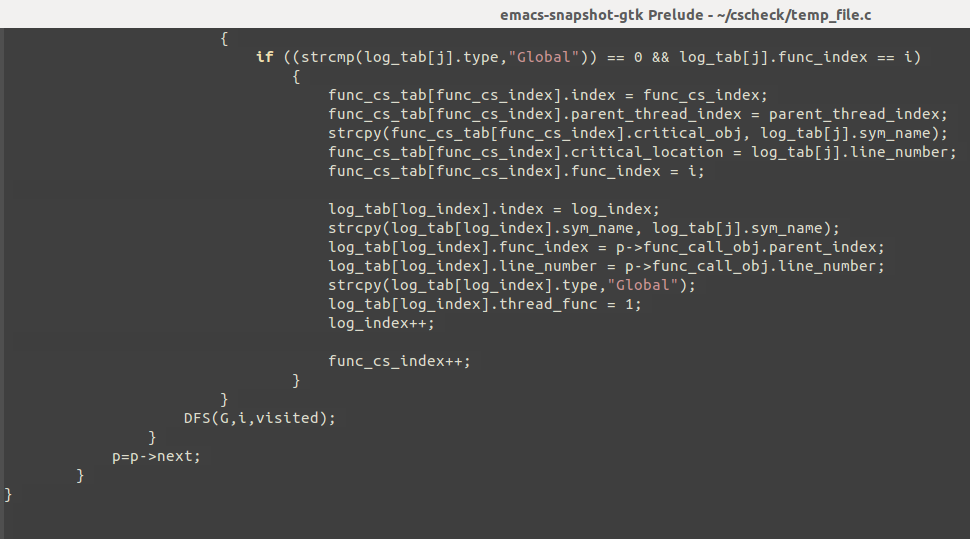
\includegraphics[scale=0.4]{Snaps/util_9.png}
\label{<<Label>>}
\end{figure}

\begin{figure}[H]
\centering
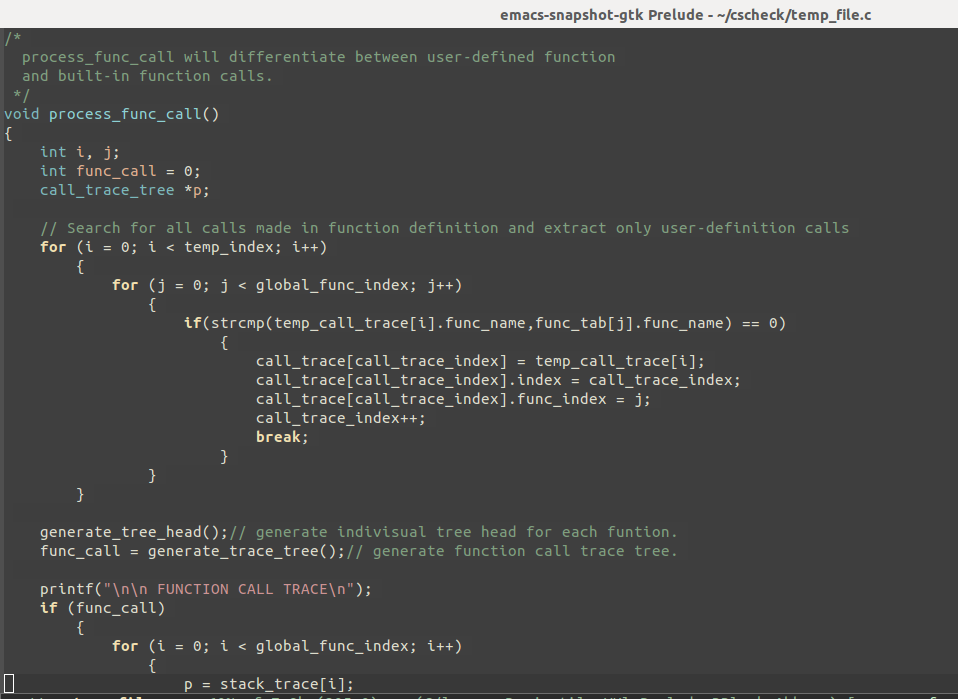
\includegraphics[scale=0.4]{Snaps/util_10.png}
\label{<<Label>>}
\end{figure}

\begin{figure}[H]
\centering
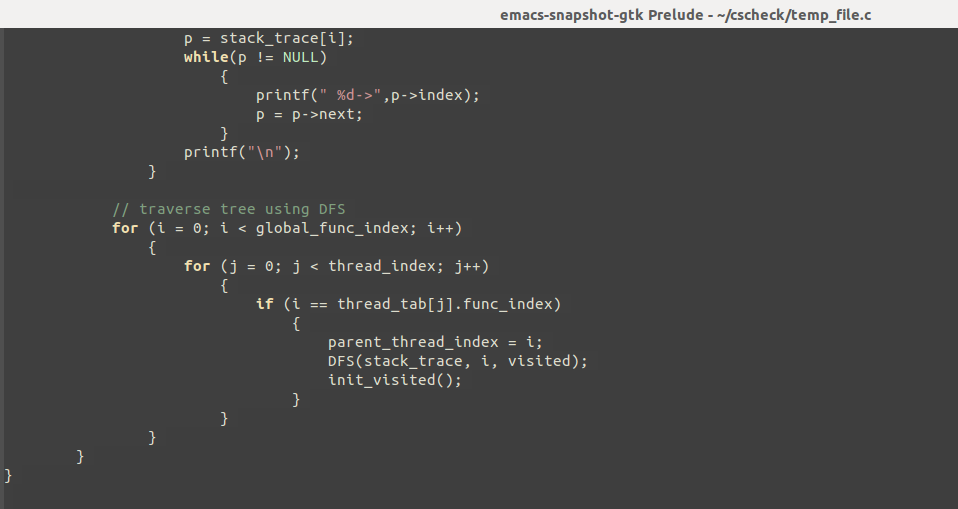
\includegraphics[scale=0.4]{Snaps/util_11.png}
\label{<<Label>>}
\end{figure}
\begin{figure}[H]
\centering
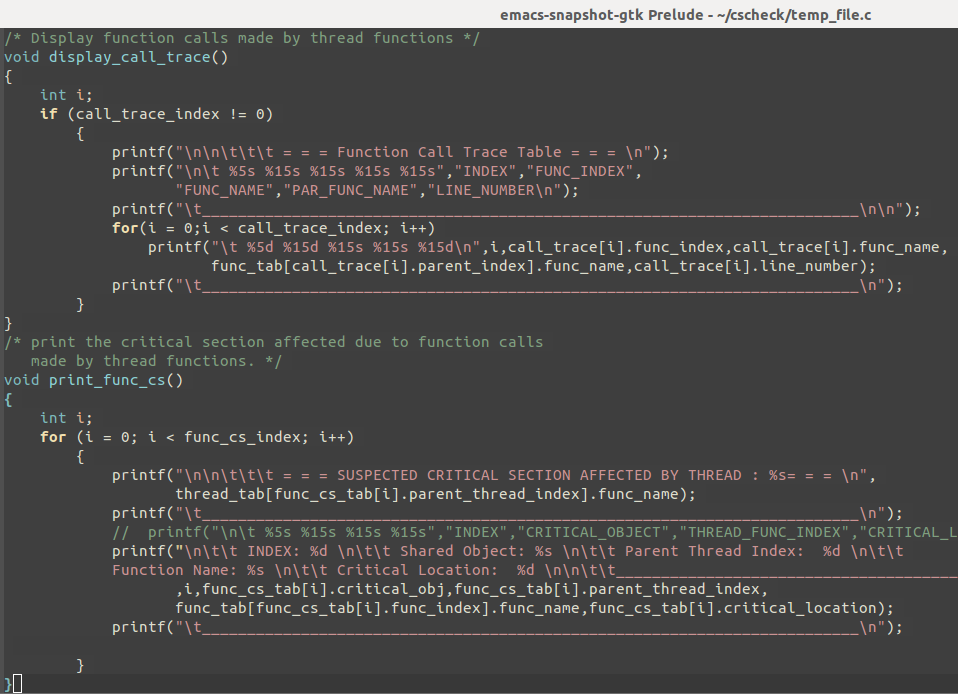
\includegraphics[scale=0.4]{Snaps/util_12.png}
\label{<<Label>>}
\end{figure}

\begin{figure}[H]
\centering
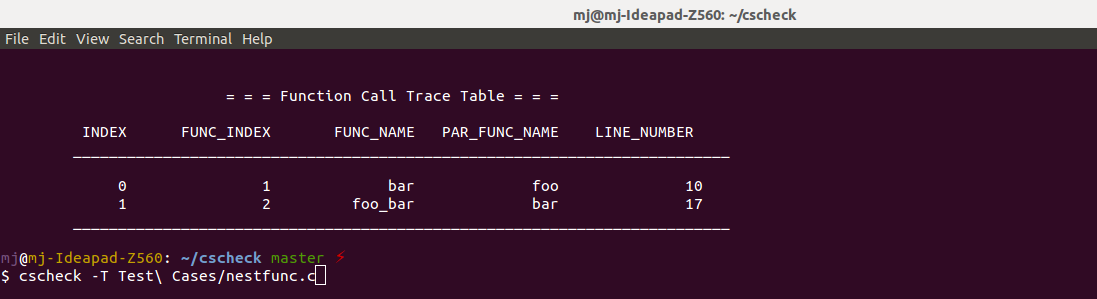
\includegraphics[scale=0.4]{Snaps/util_5-12_out1.png}
\label{<<Label>>}
\end{figure}
\begin{figure}[H]
\centering
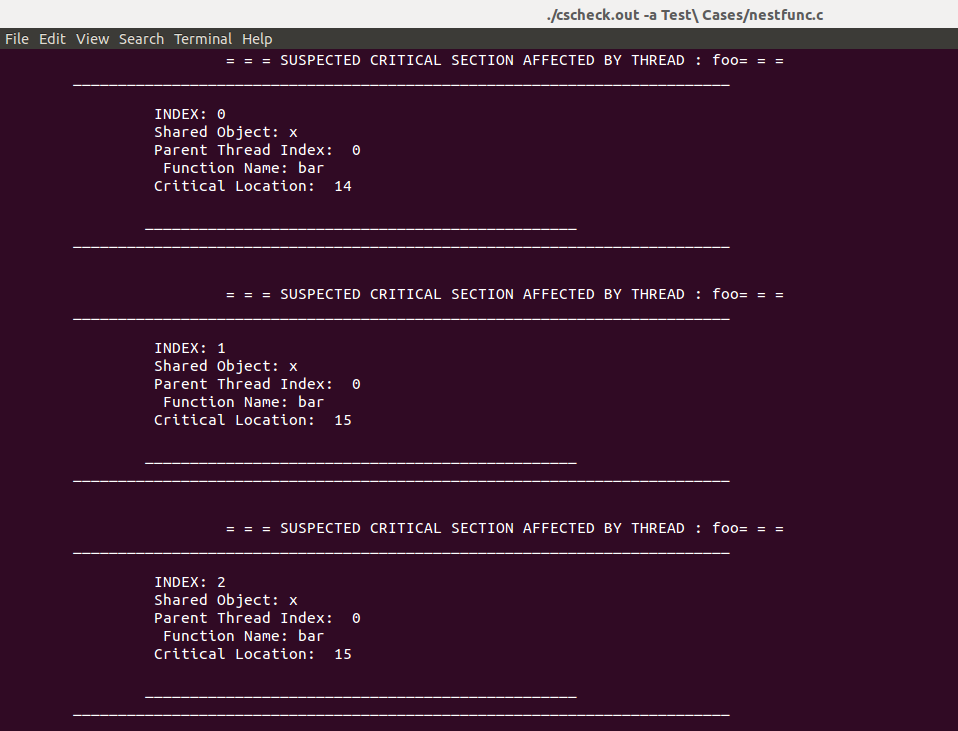
\includegraphics[scale=0.4]{Snaps/util_5-12_out2.png}
\label{<<Label>>}
\end{figure}

\begin{figure}[H]
\centering
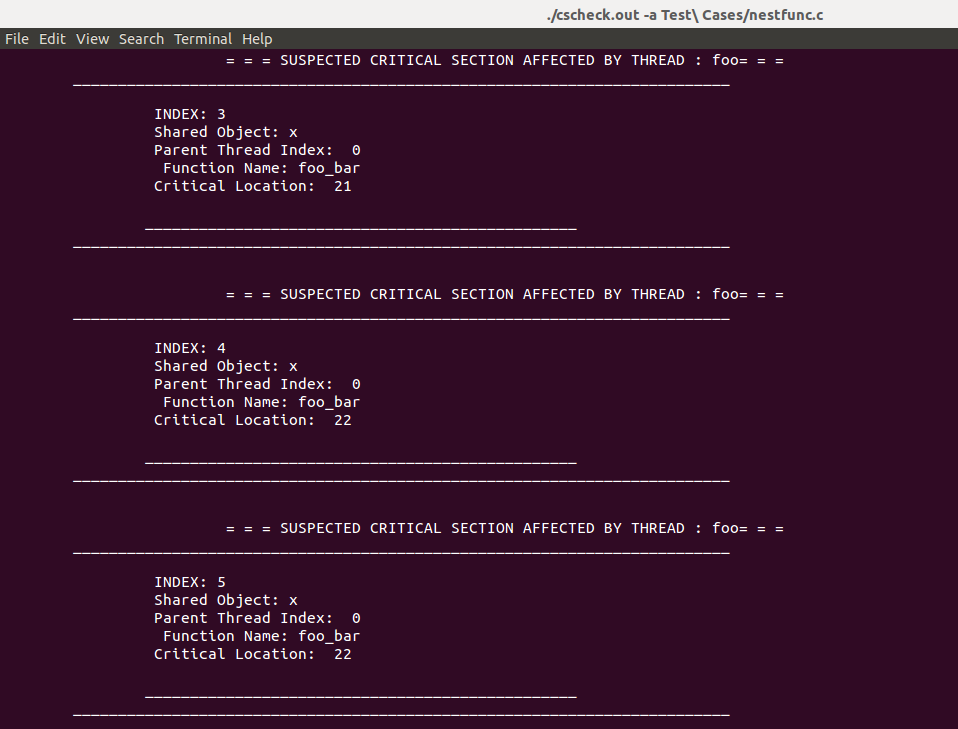
\includegraphics[scale=0.4]{Snaps/util_5-12_out3.png}
\caption{ Handling of Function call trace }
\label{<<Label>>}
\end{figure}

\begin{figure}[H]
\centering
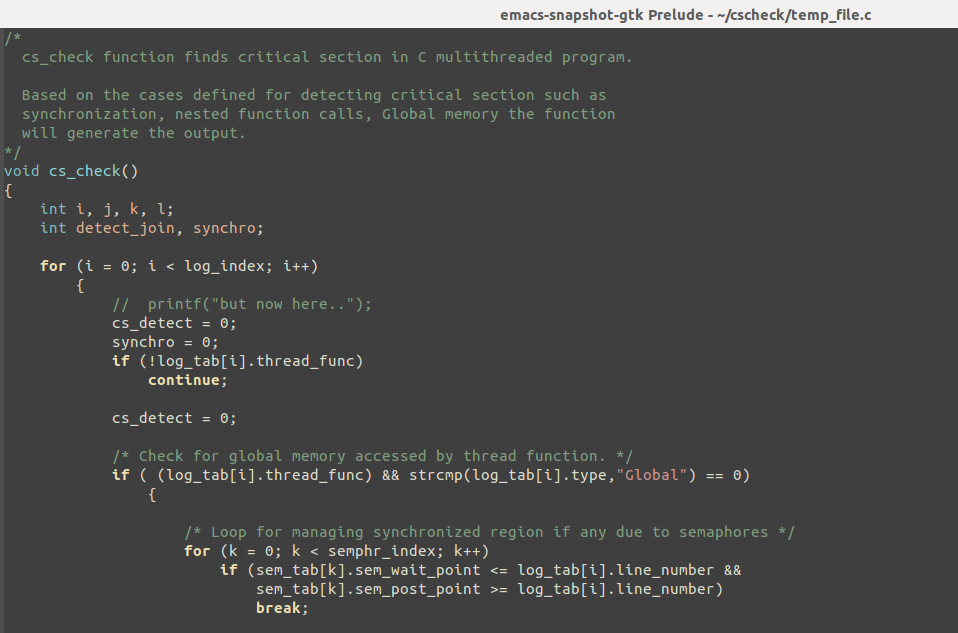
\includegraphics[scale=0.4]{Snaps/util_15.png}
\label{<<Label>>}
\end{figure}

\begin{figure}[H]
\centering
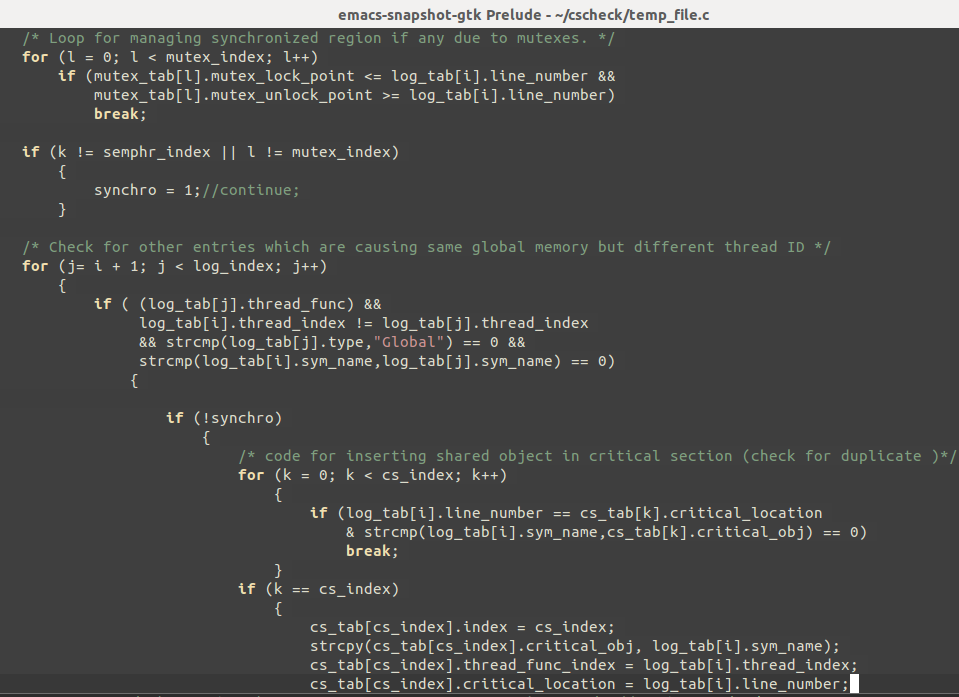
\includegraphics[scale=0.4]{Snaps/util_16.png}
\label{<<Label>>}
\end{figure}

\begin{figure}[H]
\centering
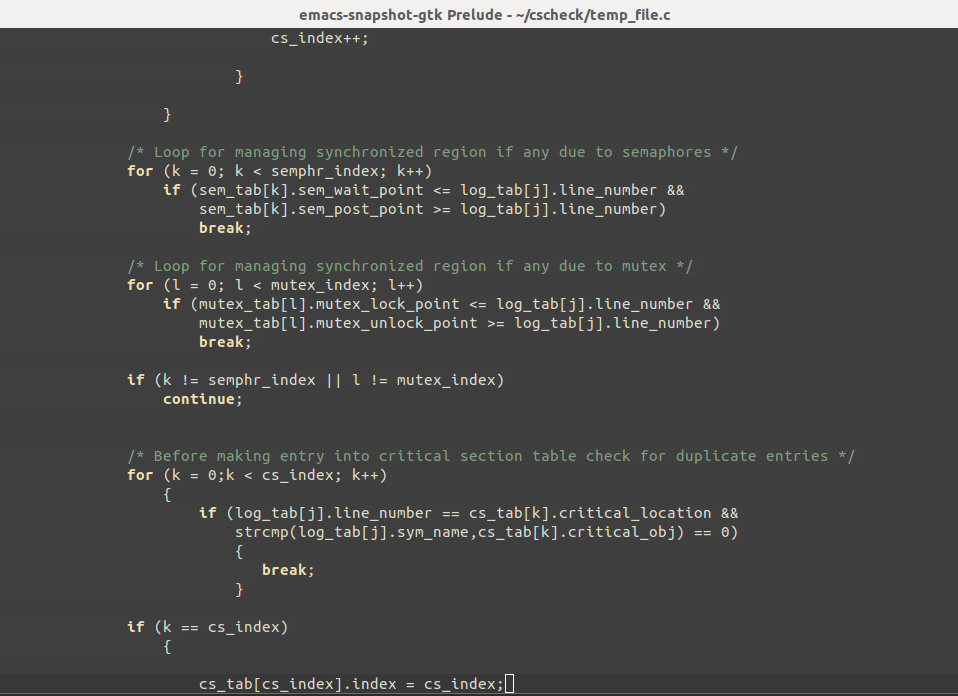
\includegraphics[scale=0.4]{Snaps/util_17.png}
\label{<<Label>>}
\end{figure}

\begin{figure}[H]
\centering
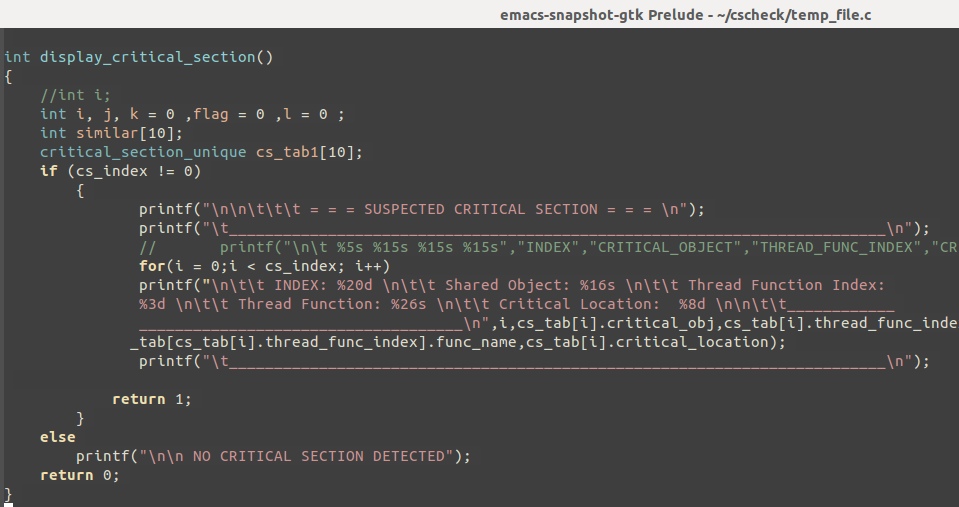
\includegraphics[scale=0.4]{Snaps/util_18.png}
\label{<<Label>>}
\end{figure}

\begin{figure}[H]
\centering
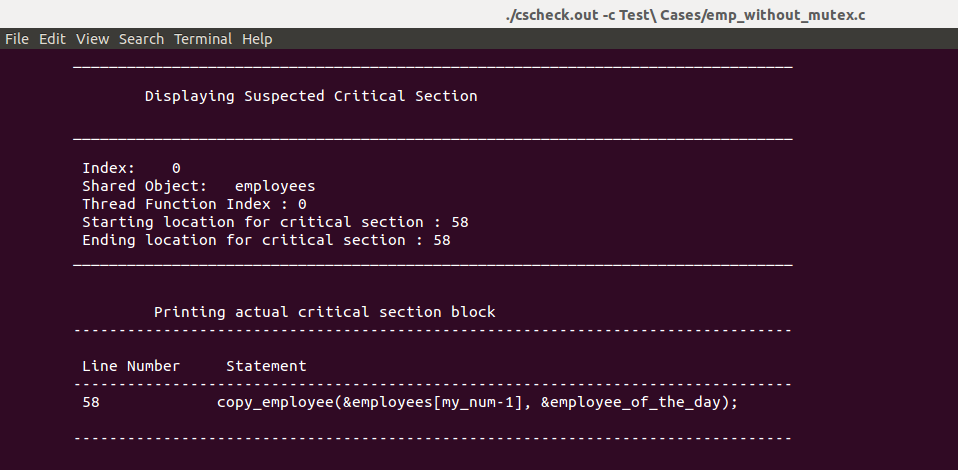
\includegraphics[scale=0.4]{Snaps/util_15-18_out1.png}
\caption{ Critical Section Detection }
\label{<<Label>>}
\end{figure}


\section{Output}
%Add Description here..\begin{itemize}
\begin{figure}[H]
\centering
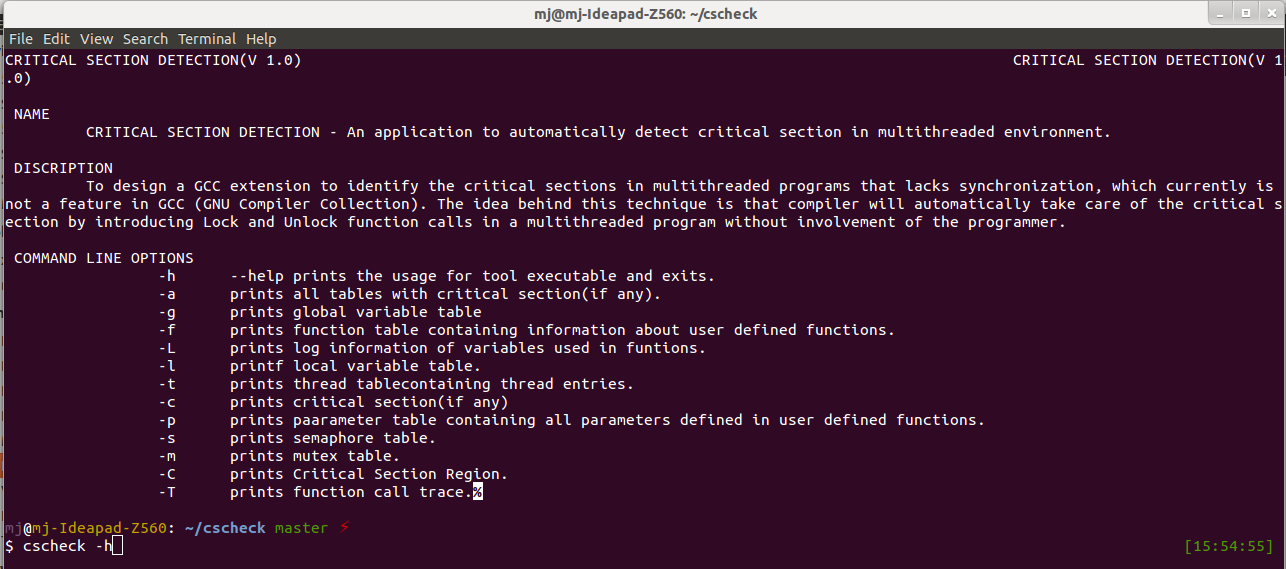
\includegraphics[scale=0.4]{Snaps/help.png}
\label{<<Label>>}
\end{figure}


\begin{figure}[H]
\centering
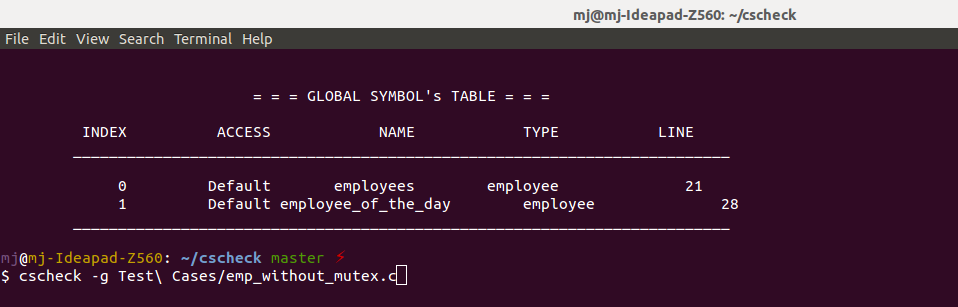
\includegraphics[scale=0.4]{Snaps/util_13-14_out1.png}
\label{<<Label>>}
\end{figure}
\begin{figure}[H]
\centering
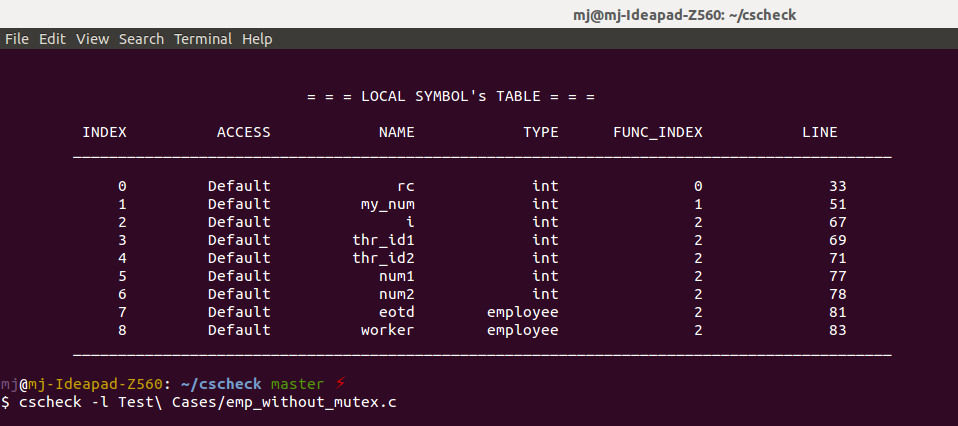
\includegraphics[scale=0.4]{Snaps/util_13-14_out2.png}
\label{<<Label>>}
\end{figure}
\begin{figure}[H]
\centering
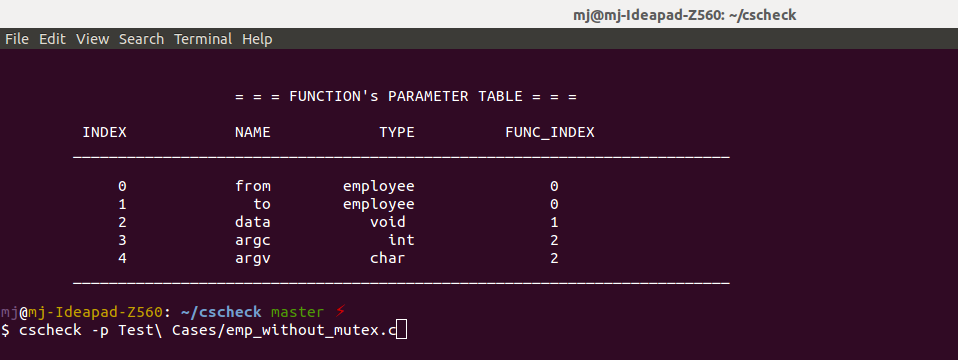
\includegraphics[scale=0.4]{Snaps/util_2_out.png}
\label{<<Label>>}
\end{figure}

\begin{figure}[H]
\centering
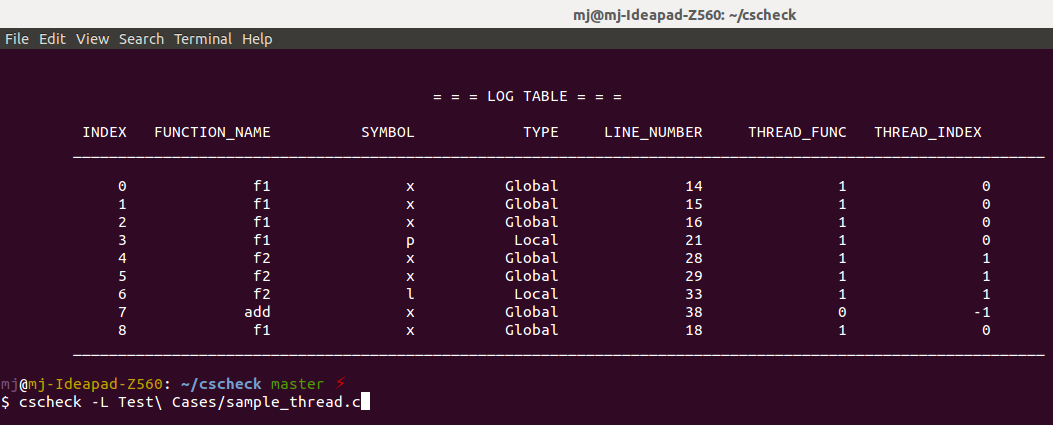
\includegraphics[scale=0.4]{Snaps/util_3_out.png}
\label{<<Label>>}
\end{figure}

\begin{figure}[H]
\centering
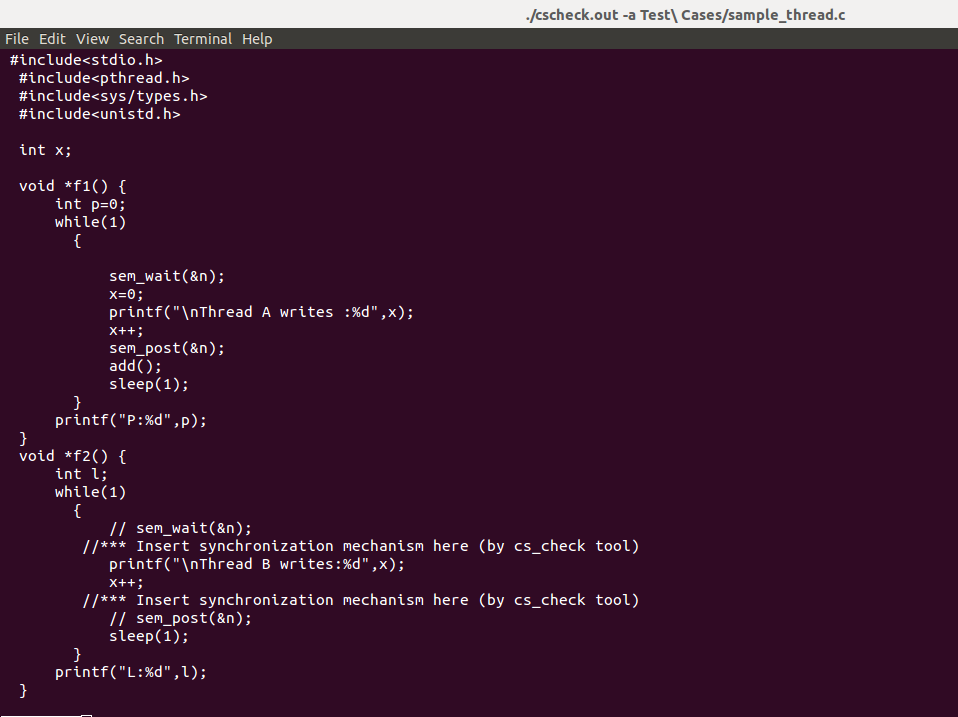
\includegraphics[scale=0.4]{Snaps/lckunlck_comment.png}
\caption{ Output }
\label{<<Label>>}
\end{figure}



\section{Testing}

% ACTUAL TABLE CODE
\setlength{\tabcolsep}{10pt}
\renewcommand{\arraystretch}{1.6}
\begin{longtable}{| p{1.9cm} | p{2.0cm} | >{\centering\arraybackslash}m{0.7cm} | p{2.1cm} | p{2.1cm} | p{1.5cm} | p{0.8cm} | }
\label{<<Label>>}
\caption{Test Cases}
\label{<<Label>>}
\hline
TestCase ID&Objective&Case&Procedure&Expected Results&Actual Results&Pass /Fail\\
\hline
\endfirsthead
\multicolumn{7}{c}%
{\tablename\ \thetable\ -- \textit{Continued from previous page}} \\
\hline
TestCase ID&Objective&Case&Procedure&Expected Results&Actual Results&Pass /Fail\\
\hline
\endhead
\hline \multicolumn{7}{r}{\textit{Continued on next page}} \\
\endfoot
\hline
\endlastfoot
Check Tools		& To check requirements of different tools. & 1. & a) Open Terminal and enter gcc. & GCC should be available.  & Same as Expected  & Pass \\
		&		&   & b) Open terminal and enter lex  & lex should be available   & Same as Expected   &  Pass  \\ 
		&		&   & c) Open terminal and enter yacc & yacc should be available   & Same as Expected   &  Pass  \\ \hline
  
Program Structure & To check nature of program. & 1. & a) Program should be errorless. & Compilation of program should be successful  & Same as Expected  & Pass \\
		&		&   & b) Program should contains POSIX threads. & Program should create new threads using POSIX API.   & Same as Expected   &  Pass  \\ \hline 

Tokenization & To create different tokens as per constraints. & 1. & a) Datatypes & Different tokens should be generated according to datatypes.  & Same as Expected  & Pass \\  
	     & & 2. & a) Function signature should be tokenized. & Fuction name,number of argument and return type should be tokenized  & Same as Expected  & Pass \\
	     & & 3. & b) POSIX thread's signature should be tokenized. & Thread object,Function name which is executed by thread,number of argument and return type should be tokenized  & Same as Expected  & Pass \\	
	     & & 4. & c) Semaphore signature should be tokenized. & Semaphore name,different semaphore signals should be tokenized  & Same as Expected  & Pass \\
     	     & & 5. & d) mutex signature should be tokenized. & Mutex name,different mutex signals should be tokenized  & Same as Expected  & Pass \\ \hline
	
Parsing & Generate different grammer as per tokens. & 1. & a) Grammer for variable datatypes. & Valid grammer should be generated for datatype.  & Same as Expected  & Pass \\  
	     & & 2. & b) Grammer for function signature. & Valid grammer should be generated for functions. & Same as Expected  & Pass \\
	     & & 3. & c) Grammer for POSIX thread's signature. & Valid grammer should be generated for threads. & Same as Expected  & Pass \\	
	     & & 4. & d) Grammer for API of Semaphore. & Valid grammer should be generated for semaphores & Same as Expected  & Pass \\
     	     & & 5. & e) Grammer for Mutex. & Valid grammer should be generated for mutex & Same as Expected  & Pass \\ \hline

Table Generation.& Different table are genereted according grammers. & 1. & a) Table for variable including global and local. & Valid tables should be generated for datatype including local and global.  & Same as Expected  & Pass \\  
	     & & 2. & b) Table for function signature. & Valid table should be generated for functions. & Same as Expected  & Pass \\
	     & & 3. & c) Table for POSIX thread's signature. & Valid table should be generated for threads. & Same as Expected  & Pass \\	
	     & & 4. & d) Table for API of Semaphore. & Valid table should be generated for semaphores & Same as Expected  & Pass \\
     	     & & 5. & e) Table for shared memory (Log Table ) & Valid table should be generated for shared memory & Same as Expected & Pass \\
             & & 6. & f) Table for Mutex. & Valid table should be generated for mutex & Same as Expected  & Pass \\ \hline 

Analysis of critical section.& Critical sections blocks are detected  & 1.& a) Locking and unlocking mechanism. & Check wheter locking and unlocking mechanism is exist for Critical Section.  & Same as Expected  & Pass \\  
	     & & 2. & b) Critical Section detection.& If critical section isn't synchronized then add it. & Same as Expected  & Pass \\ \hline

		
		 

\end{longtable}
% ACTUAL TABLE CODE END
